\section{Weitere Beispielsysteme}
\begin{frame}{Weitere Beispiele der Arbeitsgruppe Howell}
    In einer weiteren Ver\"offentlichung \cite{rochester2} sind andere kosteng\"unstige Beispiele dargestellt.
    \begin{figure}
        \centering
        \begin{subfigure}{0.48\textwidth}
            \centering
            \caption{Skizze des Systems.}
            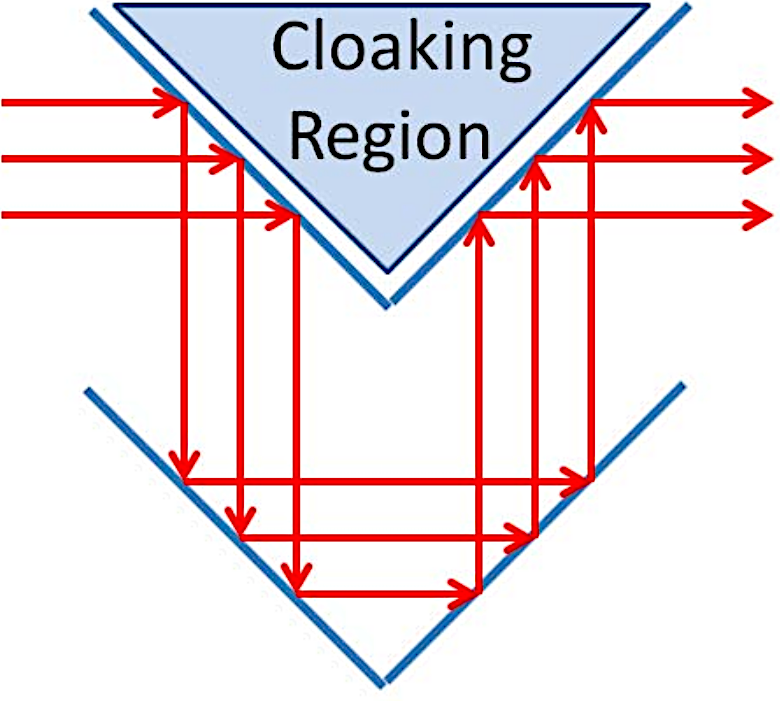
\includegraphics[height=0.6\textheight]{images/spiegel-skizze.png}
        \end{subfigure}
        \begin{subfigure}{0.48\textwidth}
            \centering
            \caption{Frontansicht des Systems.}
            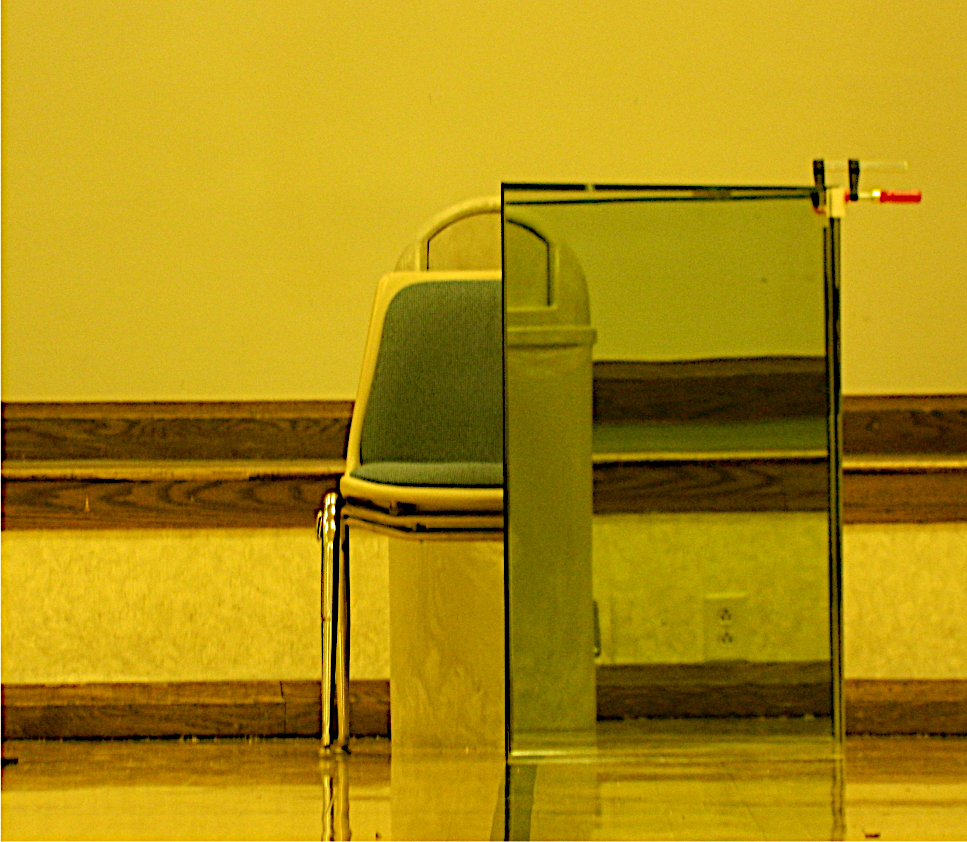
\includegraphics[height=0.6\textheight]{images/spiegel-vorne.png}
        \end{subfigure}
        \caption{Eine Tarnung aus Spiegeln.}
    \end{figure}
\end{frame}

\begin{frame}{Ein weiteres 'Linsensystem'}
    \begin{columns}
        \begin{column}{0.48\textwidth}
            \begin{figure}
                \centering
                \begin{subfigure}{\textwidth}
                    \centering
                    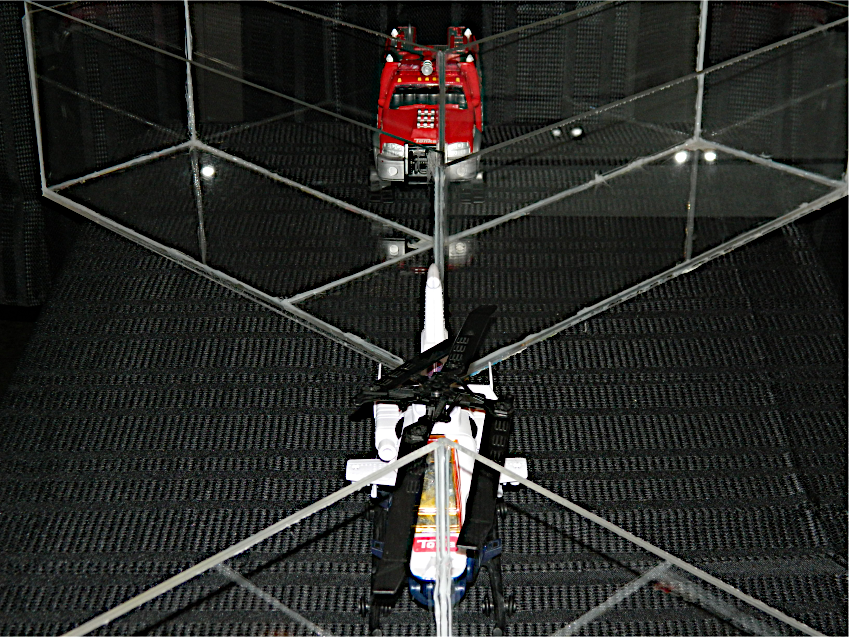
\includegraphics[height=0.4\textheight]{images/fresnel-oben.png}
                \end{subfigure}
                \begin{subfigure}{\textwidth}
                    \centering
                    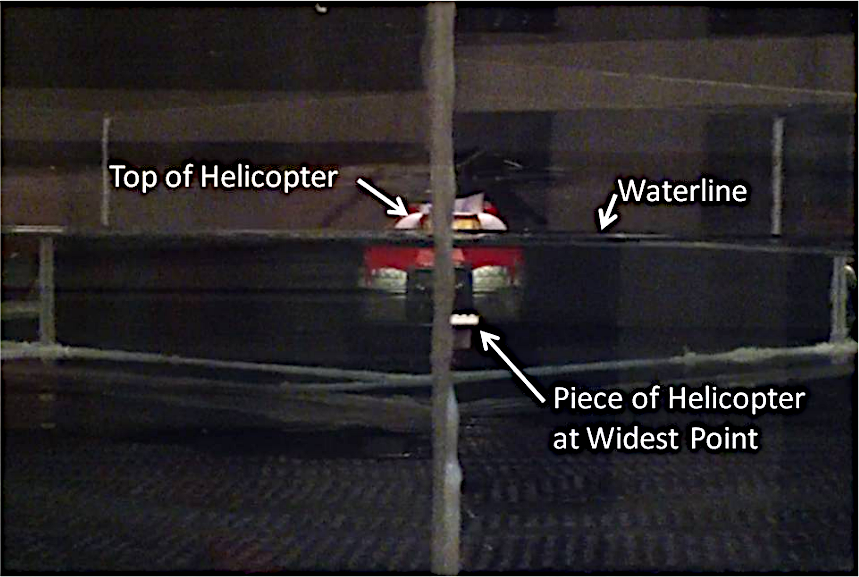
\includegraphics[height=0.4\textheight]{images/fresnel-vorne.png}
                \end{subfigure}
                \caption{Eine Tarnung mit Wasser.}
            \end{figure}
        \end{column}
        \begin{column}{0.48\textwidth}
            \begin{figure}
                \centering
                \caption{Skizze des Systems}
                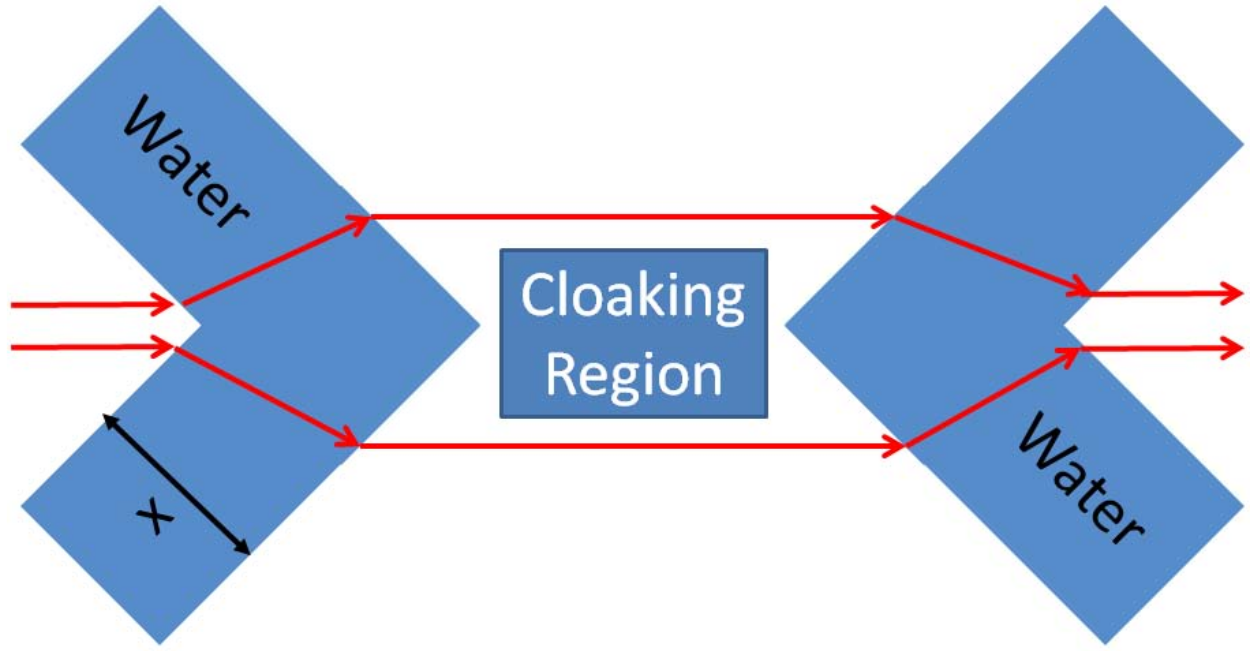
\includegraphics[height=0.3\textheight]{images/fresnel-skizze.png}
            \end{figure}
        \end{column}
    \end{columns}
\end{frame}
